\documentclass{beamer}
\usetheme{Madrid} % Professional theme recommended in slides [cite: 302, 305]
\usepackage{tikz}

\title{Summary: Designing Markets}
\subtitle{Handbook of Market Design - Chapter 4}
\author{Mohammed Alyahya}
\date{\today}

\begin{document}

\begin{frame}
    \titlepage % Generates the title slide [cite: 88, 247]
\end{frame}

\begin{frame}{What is Market Design?}
    \begin{itemize}
        \item Market design is the process of creating rules and procedures for transactions.
        \item It aims to solve specific failures in existing or new markets.
        \item Success is measured by how well the design facilitates efficient outcomes.
    \end{itemize}
    \vspace{1em}
    \textbf{Example:} Auction design for spectrum allocation, school choice mechanisms, and kidney exchange programs.
    \vspace{0.5em}
    \textbf{Key Question:} How do we create rules that encourage participation and honest behavior?
\end{frame}

% Placeholder for Exercise 1
\begin{frame}{Diagnosing Market Failures}
    \begin{itemize}
        \item Initial thoughts on congestion and thickness.
        \item Why do some markets fail to attract enough participants?
        \item What happens when too many transactions occur at once?
    \end{itemize}
    \vspace{1em}
    \textbf{Example:} Residency match programs before redesign suffered from congestion and lack of thickness.
\end{frame}

\begin{frame}{Diagnosing Market Failures (Exercise 1 Placeholder)}
    \textbf{Diagnosing Market Failures}\\[1em]
    \begin{itemize}
        \item Markets fail when they lack thickness or become too congested to function.
    \end{itemize}
    \vspace{1em}
    % Example Venn diagram for market failures
    \begin{center}
    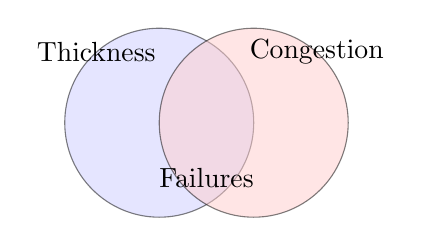
\begin{tikzpicture}
        \draw[fill=blue!20, opacity=0.5] (0,0) circle (1.2);
        \draw[fill=red!20, opacity=0.5] (1.2,0) circle (1.2);
        \node at (-0.8,0.9) {Thickness};
        \node at (2,0.9) {Congestion};
        \node at (0.6,-0.7) {Failures};
    \end{tikzpicture}
    \end{center}
\end{frame}

\begin{frame}{The Challenge of Thickness}
    \textbf{Achieving Market Thickness}\\[1em]
    \begin{itemize}
        \item A "thick" market has many potential matches at the same time.
        \item Designers must encourage participation and prevent "early" or "exploding" offers that thin out the market.
        \item Coordination of timing is crucial for maximizing options.
    \end{itemize}
    \vspace{1em}
    \textbf{Example:} School admissions deadlines and centralized matching increase thickness.
\end{frame}

\begin{frame}{Managing Congestion}
    \textbf{Overcoming Congestion}\\[1em]
    \begin{itemize}
        \item Congestion occurs when there is not enough time for participants to evaluate all offers.
        \item Designing rules to handle the volume of transactions is critical for stability.
        \item Automated systems and clear deadlines help reduce congestion.
    \end{itemize}
    \vspace{1em}
    \textbf{Example:} Electronic trading platforms in financial markets speed up transactions and reduce bottlenecks.
\end{frame}

\begin{frame}{Making Markets Safe}
    \textbf{Strategic Safety and Incentives}\\[1em]
    \begin{itemize}
        \item Participants should not be penalized for being "honest" about their preferences.
        \item Stable matching mechanisms (like Gale-Shapley) help ensure safety and commitment.
        \item Incentive compatibility is key for trust in the market.
    \end{itemize}
    \vspace{1em}
    % Example matching diagram for safety
    \begin{center}
    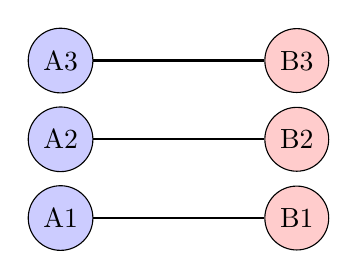
\begin{tikzpicture}[scale=1]
        \foreach \i in {1,...,3} {
            \node[circle,draw,fill=blue!20] (A\i) at (0,\i) {A\i};
            \node[circle,draw,fill=red!20] (B\i) at (3,\i) {B\i};
            \draw[thick] (A\i) -- (B\i);
        }
    \end{tikzpicture}
    \end{center}
    \vspace{0.5em}
    \textbf{Example:} The National Resident Matching Program uses stable matching to ensure safety for medical graduates.
\end{frame}

\begin{frame}{Evaluating and Comparing Designs (Exercise 2 Placeholder)}
    \textbf{Evaluating and Comparing Designs}\\[1em]
    \begin{itemize}
        \item Comparing different mechanisms involves looking at efficiency, stability, and fairness.
        \item Trade-offs: Sometimes improving one aspect reduces another (e.g., efficiency vs. fairness).
        \item Simulation and data analysis help evaluate outcomes before implementation.
    \end{itemize}
    \vspace{1em}
    \textbf{Example:} Comparing school choice algorithms for different cities to find the best fit for local needs.
\end{frame}

\begin{frame}{Applications of Market Design}
    \textbf{Real-World Applications}\\[1em]
    \begin{itemize}
        \item Labor markets (e.g., Medical Residencies).
        \item School choice systems.
        \item Kidney exchanges and organ donation networks.
        \item Online advertising auctions.
        \item Ride-sharing and gig economy platforms.
    \end{itemize}
    \vspace{1em}
    \textbf{Case Study:} Kidney exchange programs use algorithms to maximize the number of transplants.
\end{frame}

\begin{frame}{Conclusion}
    \textbf{Summary of Design Principles}\\[1em]
    \begin{itemize}
        \item Effective design requires constant diagnosis and iteration.
        \item AI tools can assist in simulating and verifying these market rules.
        \item Collaboration between economists, engineers, and policymakers is essential.
        \item Future directions: Using machine learning to optimize market rules and predict outcomes.
    \end{itemize}
    \vspace{1em}
    \textbf{Thank you for your attention! Questions?}
\end{frame}

\end{document}